 \documentclass[12pt]{article}
\usepackage[a4paper, margin=.30in]{geometry}

\usepackage{array}
\usepackage{graphicx, subfig, wrapfig, fancyhdr, lastpage,makecell }
\newcommand\headerMe[2]{\noindent{}#1\hfill#2}
\usepackage[mathscr]{euscript}



\pagestyle{fancy}
\fancyhf{}

\rfoot{\em{Page \thepage \hspace{1pt} / \pageref{LastPage}}}
\begin{document}

\headerMe{Royaume du Maroc}{année scolaire \emph{2024-2025}}\\
\headerMe{Ministère de l'Éducation nationale, }{  Professeur :\emph{Zakaria Haouzan}}\\
\headerMe{du Préscolaire et des Sports}{Établissement : \emph{Lycée SKHOR qualifiant}}\\

\begin{center}

    \vspace{-1.5cm}
Devoir  N°2 \\
   Filière Tronc Commun Scientifique\\
Durée 2h00
\\
\hrulefill
\Large{Chimie 7pts - 36min}
\hrulefill\\

    %\emph{Les Trois parties sont indépendantes}
\end{center}
%end Headerss------------------------
 
    \vspace{-1.2cm}
    
\section*{Le modèle de l'atome  \dotfill (7pts) }
%\begin{wrapfigure}[5]{r}{0.36\textwidth}
    %\vspace{-1.8cm}
    %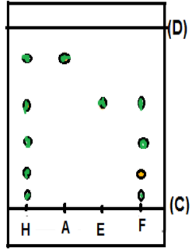
\includegraphics[width=0.36\textwidth]{./img/CCM.png}
%\end{wrapfigure}


On considère la molécule suivante de Chlorométhane $CH_3Cl$

\begin{enumerate}

\item Donner la structure électronique de carbone $C (Z=6)$, d’hydrogène $H (Z=1)$, et de chlore $Cl (Z=17)$ \dotfill(1pt)
\item  Donner le nombre $n_t$ des électrons de la couche externe de chaque atome \dotfill(1pt)
\item  Déterminer parmi ces atomes, les atomes qui obéissent à la règle du duet, et les atomes qui obéissent
à la règle de l’octet\dotfill(1pt)

\item   Déterminer le nombre de doublets liants $n_l$ et non liants $n_{nl}$ pour chaque atome. \dotfill(1pts)

\item  Représenter cette molécule selon le modèle de Lewis et déduire sa représentation de Cram \dotfill(1pt)

\item Ecrire les formules développées et les schémas de Lewis de ces composés

  $O_2$, $N_2$, $C_2H_2$, $HCN$, $C_4H_8$, $C_3H_4$ et $C_3H_6O$.
.\dotfill(2pt)
\end{enumerate}





%__________________Chimie ______________________-
%%%%%%%+_+_+_+_+_+_+_+_+_Partie1

%_____________________________________PHYSIque Partie 22222____________________________________________________________________________
\begin{center}
    \vspace{2cm}
\hrulefill
\Large{Physique 13pts - 84min}
\hrulefill\\
    \emph{Les  parties sont indépendantes}
\end{center}
%end Headerss------------------------
 \section*{Partie 1 :(la vitesse, le mouvement et le principe d'inertie) \dotfill(7pts)}

\begin{wrapfigure}[4]{r}{0.36\textwidth}
	\vspace{-0.8cm}
	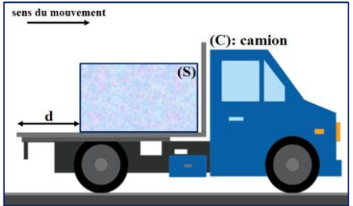
\includegraphics[width=0.36\textwidth]{./img/camion.png}
\end{wrapfigure}


Un camion (C) circulant sur une route rectiligne et horizontale,
transporte sur son plateau lisse un morceau de glace (S) de masse
$m = 20kg$. Le camion roule à vitesse constante $V_0 = 36km/h$. Le
morceau de glace reste immobile au milieu du plateau.
\vspace{1cm}
\begin{enumerate}
  \item Faire l'inventaire des forces qui agissent sur le solide (S).\dotfill(2pt)
  \item  Décrire le mouvement du morceau de glace dans un référentiel
lié au camion.\dotfill(1pt)
\item  Décrire le mouvement du morceau de glace dans un référentiel lié à la route.
A un instant $t_1$, le camion a soudainement changé sa vitesse de $V_0$ à $V_1 = 3.V_0$, pendant la durée
    $\Delta{t}=0,1s$, puis il garde plus tard sa vitesse $V_1$.\dotfill(1pt)
  \item  Pour le camion, est-ce que Le principe d’inertie vérifier pendant la durée $\Delta{t}$? Justifier ta réponse.\dotfill(1pt)

\item  Pour le morceau de glace, est-ce que Le principe d’inertie vérifier pendant la durée $\Delta{t}$? Justifier.\dotfill(0,5pt)
\item Trouver la vitesse du morceau de glace par rapport le camion et leur sens de mouvement pendant la
  durée $\Delta{t}$.\dotfill(0,5pt)
\item Sachant que le morceau de glace se trouve à d = 1,5m de l'arrière du camion à l’instant $t_1$. Le
morceau de glace tombe-t-elle du camion?\dotfill(1pt)

\end{enumerate}

\section*{Partie 2 : Vérification du concept d'inertie. \dotfill(3pts)}

\begin{wrapfigure}[4]{r}{0.36\textwidth}
	\vspace{-0.8cm}
	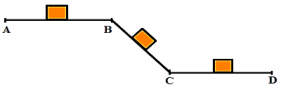
\includegraphics[width=0.36\textwidth]{./img/last.png}
\end{wrapfigure}


Un corps (S) se déplace sur un rail composé de 3 parties. On
lance ce corps du point A avec une vitesse $V_A=1m/s$ , et arrive au point D avec une vitesse $V_D=2m/s$. 

On considère que le contact se fait sans frottement.

\begin{enumerate}
	\item Faire l’inventaire des forces appliquées sur le corps (S), et représenter ces forces sur la figure pour
chaque partie. \dotfill(1pt)
\item Déterminer la partie où le principe d’inertie n’est pas vérifié.\dotfill(1pt)
\item Quelle est la valeur de la vitesse du corps (S) au point B, et au point C ? justifier votre réponse.\dotfill(1pt)
\end{enumerate}

\section*{Partie 2 : Le centre d'inertie. \dotfill(3pts)}

\begin{wrapfigure}[4]{r}{0.36\textwidth}
	\vspace{-0.8cm}
	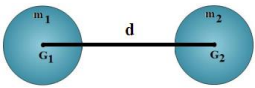
\includegraphics[width=0.36\textwidth]{./img/ex3.png}
\end{wrapfigure}


Deux sphères (A) et (B) de masses respectives $m_1$=$1kg$ et $m_2$=$3kg$ et de centres d’inertie respectives $G_1$ et $G_2$ qui sont séparés par la distance $d = 40 cm$. Ces deux sphères sont liées rigidement et constitue un système comme l’indique la figure ci-contre.

\begin{enumerate}

\item Rappeler la relation barycentrique.\dotfill(1pt)
\item Déterminer le centre d’inertie G de ce solide.\dotfill(1pt)
\item Une plaque homogène et d’épaisseur constante, et formée d’une partie carrée et de côté $a=4cm$, et d’une partie triangulaire équilatérale.

	Sachant que \textbf{la masse} de la partie triangulaire est \textbf{3 fois plus légère} que la masse de la partie carrée.

	déterminer la position du centre de masse de la plaque homogène par application d’une méthode de votre choix.\dotfill(1pt)
\end{enumerate}

 \begin{center}
	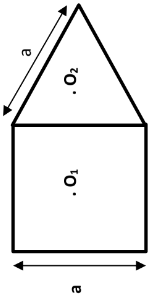
\includegraphics[width=0.16\textwidth]{./img/ex4.png}
\end{center}



\end{document}
